\chapter{Un compas suffit}\label{c.compass}




En 1797, Lorenzo Mascheroni a démontré que toute construction réalisée à la règle et au  compas peut être réalisée avec un compas seulement. Il est apparu plus tard que ce théorème avait déjà été démontré par Georg Mohr en 1672. 
Après avoir expliqué dans la section~\ref{s.compass-what} ce que signifie effectuer une construction avec seulement un compas, on présente la démonstration par étapes en commençant par quatre constructions auxiliaires : la réflexion d'un point (sect.~\ref{s.reflection}), la construction d'un cercle de rayon donné (sect.~\ref{s.circle}), l'addition et la soustraction de segments  (sect.~\ref{s.add-subtract}) et la construction d'un segment  comme rapport de segments (sect.~\ref{s.three}). La section~\ref{s.two-lines} montre comment trouver l'intersection de deux droites. La section~\ref{s.line-circle} montre comment trouver l'intersection d'une droite et d'un cercle.

\section{Qu'est-ce qu'une construction avec seulement un compas ?}\label{s.compass-what}

La figure~\ref{f.compass-equi} montre la construction d'un triangle équilatéral à l'aide d'une règle et d'un compas. Comment construire un triangle sans les segments  $\overline{AB}$, $\overline{AC}$ et $\overline{BC}$ ? Un segment  est défini par deux points, il suffit donc de construire ces points pour obtenir une construction équivalente à celle obtenue avec une règle (fig.~\ref{f.compass-equi-only}). Il n'est pas nécessaire de voir réellement les segments.
Il y aura des droites dans les figures de ce chapitre, mais elles ne servent qu'à comprendre la construction et la démonstration  de son exactitude. Il est important de se convaincre que la construction elle-même n'utilise qu'un compas.


Une construction à l'aide d'une règle et d'un compas est une suite de trois opérations :
\begin{itemize}
\item trouver le point d'intersection de deux droites.
\item trouver les points d'intersection d'une droite et d'un cercle.
\item trouver les points d'intersection de deux cercles.
\end{itemize}
La troisième opération peut être réalisée avec un simple compas. Nous devons montrer que les deux premières opérations peuvent être effectuées uniquement avec un compas. 

\vspace{0.4cm}

\begin{minipage}{0.4\textwidth}
\centering     
\begin{tikzpicture}[scale=0.6]
\coordinate (A) at (0,0);
\coordinate (B) at (4,0);
\vertex{A};
\vertex{B};
\draw (A) node[below left] {$A$} -- (B) node[below right] {$B$};
\draw[name path=larc] (A) ++(-10:4cm) arc (-10:80:4cm);
\draw[name path=rarc] (B) ++(-170:4cm) arc (-170:-260:4cm);
\path [name intersections={of=larc and rarc,by={t}}];
\node[above right,xshift=-2pt,yshift=3pt] at (t) {$C$};
\vertex{t};
\draw (A) -- (t);
\draw (B) -- (t);
\end{tikzpicture}
%\includegraphics[width=0.7\textwidth]{Fig13_1a}
         \captionof{figure}{Construction d'un triangle équilatéral avec une règle et un compas.}\label{f.compass-equi}
         
     \end{minipage}
     \hspace{3em}
     \begin{minipage}{0.4\textwidth}
\centering       
\begin{tikzpicture}[scale=0.6]
\coordinate (A) at (0,0);
\coordinate (B) at (4,0);
\vertex{A};
\vertex{B};
\path (A) node[below left] {$A$} -- (B) node[below right] {$B$};
\draw[name path=larc] (A) ++(-10:4cm) arc (-10:80:4cm);
\draw[name path=rarc] (B) ++(-170:4cm) arc (-170:-260:4cm);
\path [name intersections={of=larc and rarc,by={t}}];
\node[above right,xshift=-2pt,yshift=3pt] at (t) {$C$};
\vertex{t};
\end{tikzpicture}
%\includegraphics[width=0.7\textwidth]{Fig13_1b}
         \captionof{figure}{Construction d'un triangle équilatéral avec seulement un compas.}\label{f.compass-equi-only}
     \end{minipage}

\vspace{0.4cm}





\noindent{}Notations.
\begin{itemize}
\item $c(O,A)$: le cercle de centre $O$ qui passe par le point $A$.
\item $c(O,r)$: le cercle de centre $O$ et de rayon $r$.
\item $c(O,\overline{AB})$: le cercle de centre $O$ et de rayon égal à la longueur du segment $\overline{AB}$.
\end{itemize}

%%%%%%%%%%%%%%%%%%%%%%%%%%%%%%%%%%%%%%%%%%%%%%%%%%%%%%%%%%%%%%%

\section{Réflexion d'un point}\label{s.reflection}

\begin{definition}
Un point $C'$ est le \emph{symétrique} du point $C$ par rapport au segment  $\overline{AB}$ si  la droite contenant $\overline{AB}$ est la médiatrice du segment $\overline{CC'}$.
\end{definition}

\begin{theorem}\label{thm.compass-reflection}
Étant donné une droite $\overline{AB}$ et un point $C$ non situé sur $\overline{AB}$, il est possible de construire le symétrique $C'$ de $C$ par rapport à $\overline{AB}$.
\end{theorem}

\begin{proof} 
Construisons un cercle de centre $A$ passant par $C$ et un cercle de centre $B$ passant par $C$. L'autre intersection des deux cercles est le point $C'$ qui est le  symétrique de $C$ (fig.~\ref{f.compass-reflection}).
$\triangle ABC \cong \triangle ABC'$ (trois côtés égaux) puisque $\overline{AC}$ et $\overline{AC'}$ sont des rayons du même cercle, tout comme $\overline{BC}$ et $\overline{BC'}$, tandis que  $\overline{AB}$ est un côté commun. Par conséquent, $\angle CAB = \angle C'AB$ et donc $\overline{AB}$ est la bissectrice de $\angle CAC'$. Mais $\triangle CAC'$ est un triangle isocèle. La bissectrice  $\overline{AB}$ est aussi la médiatrice de $\overline{CC'}$, la base de $\triangle CAC'$. Par définition, $C'$ est le symétrique de $C$ par rapport à $\overline{AB}$.
\end{proof}

\begin{figure}[t]
\centering
\begin{tikzpicture}[scale=.7]
\coordinate (A) at (0,0);
\coordinate (B) at (4,0);
\coordinate (C) at (2.5,1.5);
\draw ($(B)!2!(A)$) -- ($(A)!2!(B)$);
\node[above left] at (A) {$A$};
\node[above right] at (B) {$B$};
\node[above,yshift=4pt] at (C) {$C$};
\node[draw,circle through=(C),name path=ac] at (A) {};
\node[draw,circle through=(C),name path=bc] at (B) {};
\path [name intersections={of=ac and bc,by={x1,Cp}}];
\node[below,yshift=-4pt] at (Cp) {$C'$};
\draw (C) -- (Cp);
\vertex{A};
\vertex{B};
\draw (A) -- (C);
\draw (B) -- (C);
\draw (A) -- (Cp);
\draw (B) -- (Cp);
\coordinate (center) at (2.5,0);
\draw[rotate=90] (center) rectangle +(8pt,8pt);
\end{tikzpicture}
%\includegraphics[width=\textwidth]{Fig13_2}
\caption{Construction du symétrique.}\label{f.compass-reflection}
\end{figure}


%%%%%%%%%%%%%%%%%%%%%%%%%%%%%%%%%%%%%%%%%%%%%%%%%%%%%%%%%%%%%%%



\section{Construction d'un cercle de rayon donné}\label{s.circle}

\begin{theorem}\label{thm.compass-radius}
Étant donné les points $A$, $B$ et $C$, il est possible de construire $c(A,\overline{BC})$, le cercle de centre $A$ et de rayon $\overline{BC}$.
\end{theorem}

\begin{proof}
Construisons $c(A,B)$ et $c(B,A)$. Soient $X$ et $Y$  leurs points d'intersection (fig.~\ref{f.compass-circle1}). $A$ est le symétrique de $B$ par rapport à $\overline{XY}$ puisque $\triangle YAX\cong \triangle YBX$ (trois côtés égaux). Avec le théorème~\ref{thm.compass-reflection}, on construit le symétrique $C'$ de $C$ par rapport à $\overline{XY}$ et ensuite on construit $c(A,\overline{AC'})$ (fig.~\ref{f.compass-circle3}).

\begin{figure}[htbp]
\centering
\begin{tikzpicture}[scale=.5]
\coordinate (A) at (0,1.5);
\coordinate (B) at (0,-1.5);
\coordinate (C) at (1.5,-3);
\coordinate (Cp) at (1.5,3);
\vertex{A};
\vertex{B};
\vertex{C};
\node[above] at (A) {$A$};
\node[below] at (B) {$B$};
\node[below] at (C) {$C$};
\node[draw,circle through=(B),name path=ab] at (A) {};
\node[draw,circle through=(A),name path=ba] at (B) {};
\path [name intersections={of=ab and ba,by={Y,X}}];
\node[above right,xshift=4pt] at (X) {$X$};
\node[above left,xshift=-4pt] at (Y) {$Y$};
\draw[dashed] ($(X)!2!(Y)$) -- ($(Y)!2!(X)$);
\coordinate (Cp) at (1.5,3);
\vertex{Cp};
\node[above,yshift=2pt] at (Cp) {$C'$};
\draw (A) -- (B);
\draw (C) -- (Cp);
\draw (Y) -- (A) -- (X) -- (B) -- cycle;
\end{tikzpicture}
%\includegraphics[width=0.8\textwidth]{Fig13_3}
\caption{Construction d'un cercle avec un rayon donné (1).}\label{f.compass-circle1}
\end{figure}

$\overline{XY}$ est la médiatrice de $\overline{CC'}$ et $\overline{AB}$. Soit $D$ l'intersection de $\overline{XY}$ et de $\overline{AB}$. Soit $E$ l'intersection de $\overline{XY}$ et de $\overline{CC'}$. Alors $\overline{C'E}=\overline{EC}$, $\overline{AD}=\overline{DB}$ et $\angle DEC=\angle DEC'$ est un angle droit, donc $\triangle DEC\cong\triangle DEC'$ (deux côtés et un angle égaux). Par conséquent, $\overline{DC}=\overline{DC'}$ et $\angle ADC'=\angle BDC$ (ils sont complémentaires de $\angle EDC'=\angle EDC$). Il s'ensuit que $\triangle ADC'\cong\triangle BDC$ (deux côtés et un angle égaux).  Donc $\overline{AC'}=\overline{BC}$.
\end{proof}

\begin{figure}[htbp]
\centering
\begin{tikzpicture}[scale=.6]
\coordinate (A) at (0,1.5);
\coordinate (B) at (0,-1.5);
\coordinate (C) at (1.5,-3);
\coordinate (Cp) at (1.5,3);
\node[above,yshift=2pt] at (A) {$A$};
\node[below,yshift=-2pt] at (B) {$B$};
\node[below,yshift=-2pt] at (C) {$C$};
\node[above,xshift=1pt,yshift=2pt] at (Cp) {$C'$};
\node[circle through=(B),name path=ab] at (A) {};
\node[circle through=(A),name path=ba] at (B) {};
\path [name intersections={of=ab and ba,by={Y,X}}];
\node[above right,xshift=4pt] at (X) {$X$};
\node[above left,xshift=-4pt] at (Y) {$Y$};
%\node[draw,circle through=(C)] at (Y) {};
\draw[dashed] ($(X)!1.8!(Y)$) -- ($(Y)!1.8!(X)$);
\path[name path=xy] (X) -- (Y);
\node[draw,thick,circle through=(Cp)] at (A) {};
\draw (A) -- (Cp);
\draw (B) -- (C);
\draw[name path=abline] (A) -- (B);
\draw[name path=ccp] (C) -- (Cp);
\path[name intersections={of=xy and abline,by={D}}];
\path[name intersections={of=xy and ccp,by={E}}];
\node[above left] at (D) {$D$};
\node[below right,xshift=-3pt] at  (E) {$E$};
\draw (D) -- (Cp);
\draw (D) -- (C);
\draw (D) rectangle +(9pt,9pt);
\draw (E) rectangle +(9pt,9pt);
\vertex{Y};
\vertex{A};
\vertex{X};
\end{tikzpicture}
%\includegraphics[width=0.8\textwidth]{Fig13_4}

\caption{Construction d'un cercle avec un rayon donné (2).}\label{f.compass-circle3}
\end{figure}

%%%%%%%%%%%%%%%%%%%%%%%%%%%%%%%%%%%%%%%%%%%%%%%%%%%%%%%%%%%%%%%

\section{Addition et soustraction de segments}\label{s.add-subtract}

\begin{figure}[bhtp]
\begin{tikzpicture}[scale=.8]
\coordinate (P) at (0,0);
\coordinate (Q) at (5,0);
\coordinate (T) at (3,0);
\coordinate (U) at (7,0);
\vertex{P};
\vertex{Q};
\vertex{U};
\vertex{T};
\draw (P) -- (Q);
\node[above] at (P) {$P$};
\node[above left] at (Q) {$Q$};
\node[above left] at (U) {$U$};
\node[above right] at (T) {$T$};
\draw (5,0) -- (8,0);
\coordinate (R) at (9,-1);
\coordinate (S) at ($(9,-1) + (20:2cm)$);
\vertex{R};
\vertex{S};
\draw (R) node[above] {$R$} -- node[below right] {$b$} (S) node[above] {$S$};
\draw[<->] (0,-.5) -- node[fill=white] {$a$} (5,-.5);
\draw[<->] (0,-1) -- node[fill=white] {$a-b$} (3,-1);
\draw[<->] (0,-1.5) -- node[fill=white] {$a+b$} (7,-1.5);
\end{tikzpicture}
%\includegraphics[width=\textwidth]{Fig13_5}
\caption{Addition et soustraction de segments.}\label{f.compass-add1}
\end{figure}

\begin{theorem}\label{thm.add-subtract-mm}
Étant donné un segment $\overline{PQ}$ de longueur $a$ et un segment $\overline{RS}$ de longueur $b$, il est possible de construire des segments  $\overline{QT}$ et $\overline{QU}$ tels que $\overline{PTQU}$ soit un segment, la longueur de $\overline{PT}$ étant $a-b$ et la longueur de $\overline{PU}$ étant $a+b$  (fig.~\ref{f.compass-add1}).
\end{theorem}



La démonstration est assez longue et sera présentée comme une suite de constructions.


\begin{theorem}\label{thm.compass-trapezoid}
On peut construire un trapèze isocèle.
\end{theorem}

\begin{proof}
Soit $H$ un point quelconque sur $c(Q,b)$. Construisons son symétrique $H'$ par rapport à $\overline{PQ}$. Soit $h$ la longueur de $\overline{HH'}$  (fig.~\ref{f.compass-isoceles-trap1}).

\begin{figure}[ht]
\centering
\begin{tikzpicture}[scale=.5]
\coordinate (Q) at (0,0);
\coordinate (P) at (-6.8,0);
\coordinate (B) at (-3,-2);
\draw ($(Q)!1.3!(P)$) -- node[above,near start] {$a$} ($(P)!2.3!(Q)$);
\node[above left] at (Q) {$Q$};
\node[above] at (P) {$P$};
\node[draw,circle through=(B),name path=qb] at (Q) {};
\draw (Q) -- node[left,xshift=-1pt,yshift=2pt] {$b$} (B);
\path[name path=qh] (Q) -- (-40:5cm);
\path[name path=qhp] (Q) -- (40:5cm);
\path [name intersections={of=qb and qh,by={H}}];
\path [name intersections={of=qb and qhp,by={Hp}}];
\node[right,xshift=2pt] at (H) {$H'$};
\node[right,xshift=2pt] at (Hp) {$H$};
\draw (H) -- node[below left,yshift=-2pt] {$h$} (Hp);
\vertex{P};
\vertex{Q};
\end{tikzpicture}
%\includegraphics[width=\textwidth]{Fig13_6}
\caption{Construction d'un trapèze isocèle  (1).}\label{f.compass-isoceles-trap1}
\end{figure}

Construisons les cercles $c(H,b)$ et $c(Q,h)$. Soit $K$ un point d'intersection des cercles. Construisons le symétrique $K'$  de $K$ par rapport à $\overline{PQ}$ (fig.~\ref{f.compass-isoceles-trap2}).

\begin{figure}[htbp]
\centering
\begin{tikzpicture}[scale=.5]
\coordinate (Q) at (0,0);
\coordinate (P) at (-6.8,0);
\coordinate (B) at (-3,-2);
\draw ($(Q)!1.3!(P)$) -- ($(P)!2.3!(Q)$);
\vertex{Q};
\vertex{P};
\node[above right,xshift=7pt] at (Q) {$Q$};
\node[above] at (P) {$P$};
\node[draw,circle through=(B),name path=qb] at (Q) {};
\draw (Q) -- node[left,xshift=-1pt,yshift=2pt] {$b$} (B);
\path[name path=qh] (Q) -- (-40:5cm);
\path[name path=qhp] (Q) -- (40:5cm);
\path [name intersections={of=qb and qh,by={Hp}}];
\path [name intersections={of=qb and qhp,by={H}}];
\node[right,xshift=2pt] at (H) {$H$};
\node[right,xshift=2pt] at (Hp) {$H'$};
\draw (H) -- node[below left,yshift=-3pt] {$h$} (Hp);
\vertex{H};
\coordinate (Qp) at (H|-Q);
\draw (Qp) rectangle +(10pt,10pt);
\node[above left] at (Qp) {$Q'$};
\draw[name path=circleqh] (Q) let
  \p1 = ($ (H) - (Hp) $),
  \n2 = {veclen(\x1,\y1)}
in
  circle (\n2)
  (Q) edge node[below] {$h$} +(140:\n2) ++(140:\n2) coordinate (q);
\draw[name path=circlehb] (H) let
  \p1 = ($ (Q) - (B) $),
  \n2 = {veclen(\x1,\y1)}
in
  circle (\n2)
  (H) edge node[below,near end] {$b$} +(50:\n2) ++(50:\n2)  coordinate (h);
\path [name intersections={of=circleqh and circlehb,by={K}}];
\node[above left] at (K) {$K$};
\draw let
  \p1 = ($ (K) - (Q) $)
in
  coordinate (Kp) at (\x1,-\y1);
\node[below left] at (Kp) {$K'$};
\draw (K) -- (Kp);
\draw (Q) rectangle +(10pt,10pt);
\draw[dashed] (K) -- node[right,yshift=1pt] {$b$} (H) -- (Q);
\draw[dashed] (Kp) -- (Hp) -- (Q);
\end{tikzpicture}
%\includegraphics[width=\textwidth]{Fig13_7}

\caption{Construction d'un trapèze isocèle  (2).}\label{f.compass-isoceles-trap2}
\end{figure}



La droite contenant $\overline{PQ}$ est la médiatrice de $\overline{HH'}$ et $\overline{KK'}$, donc $\overline{HH'}\parallel \overline{KK'}$. $\overline{KH}=b$ puisque c'est le rayon du cercle de centre $H$. Les points $K'$ et $H'$ sont les symétriques de $K$ et $H$. $\triangle QQ'H\cong \triangle QQ'H'$ (trois côtés égaux) et $\triangle KQH\cong \triangle K'QH'$ (deux côtés et un angle égaux), donc $\overline{K'H'}=\overline{KH}=b$. Il s'ensuit que $\overline{KHH'K'}$ est un trapèze isocèle dont les bases sont $\overline{HH'}=h$ et $\overline{KK'}=2h$ (fig.~\ref{f.compass-isoceles-trap3}). On note  $d$ la longueur des diagonales $\overline{K'H}=\overline{KH'}$.
\end{proof}

\begin{figure}[htbp]
\centering
\begin{tikzpicture}[scale=.5]
\coordinate (Q) at (0,0);
\coordinate (P) at (-6.8,0);
\coordinate (B) at (-3,-2);
\draw[dashed] ($(Q)!1.3!(P)$) -- ($(P)!2.3!(Q)$);
\node[above left] at (Q) {$Q$};
\node[above] at (P) {$P$};
\vertex{P};
\vertex{Q};
\node[draw,circle through=(B),name path=qb] at (Q) {};
\path[name path=qh] (Q) -- (-40:5cm);
\path[name path=qhp] (Q) -- (40:5cm);
\path [name intersections={of=qb and qh,by={Hp}}];
\path [name intersections={of=qb and qhp,by={H}}];
\node[right,xshift=2pt] at (H) {$H$};
\node[right,xshift=2pt] at (Hp) {$H'$};
\draw (H) -- node[below right,yshift=-2pt] {$h$} (Hp);
\path[name path=circleqh] (Q) let
  \p1 = ($ (H) - (Hp) $)
in
  circle ({veclen(\x1,\y1)});
\path[name path=circlehb] (H) let
  \p1 = ($ (Q) - (B) $)
in
  circle ({veclen(\x1,\y1)});
\path [name intersections={of=circleqh and circlehb,by={K,k2}}];
\node[above left] at (K) {$K$};
\draw (Q) -- node[left] {$h$} (K);
\draw (H) -- node[right,xshift=4pt] {$b$} (K);
\draw let
  \p1 = ($ (K) - (Q) $)
in
  coordinate (Kp) at (\x1,-\y1);
\node[below left] at (Kp) {$K'$};
\draw (Q) -- node[left] {$h$} (Kp) -- node[right,xshift=2pt,yshift=-2pt] {$b$} (Hp);
\draw (K) -- node[above right] {$d$} (Hp);
\draw (Kp) -- node[left] {$d$} (H);
\end{tikzpicture}
%\includegraphics[width=0.9\textwidth]{Fig13_8}

\caption{Construction d'un trapèze isocèle  (3).}\label{f.compass-isoceles-trap3}
\end{figure}


\begin{theorem}
Un trapèze isocèle peut être circonscrit par un cercle.
\end{theorem}

\begin{proof}
Le théorème découle immédiatement des théorèmes~\ref{thm.quad-circum} et  \ref{thm.isoceles-trapezoid}.
\end{proof}

\begin{theorem}\label{thm.ptolemy-trap}
Pour $d$, $b$ et $h$ dans la figure~\ref{f.compass-isoceles-trap3}, on a  $d^2=b^2+2h^2$.
\end{theorem}

\begin{proof}
Ceci découle du théorème de Ptolémée (théorème~\ref{thm.ptolemy}) qui dit que dans un quadrilatère circonscrit par un cercle, le produit des diagonales est égal à la somme des produits des côtés opposés.
\end{proof}

On peut maintenant présenter la démonstration du théorème~\ref{thm.add-subtract-mm}.
\begin{proof}
Soit $X$ le point de la droite $\overline{PQ}$ qui prolonge $\overline{PQ}$ par $b$ (nous construirons $X$ par la suite). Posons $x = \overline{K'X}$. D'après le théorème~\ref{thm.ptolemy-trap},
\[
d^2=b^2 + 2h^2 = (x^2-h^2)+2h^2 =x^2+h^2\,.
\]
Puisque $\triangle QK'X$ est un triangle rectangle, on a $x^2 = b^2 + h^2$ (fig.~\ref{f.compass-isoceles-trap4}).


\begin{figure}[thbp]
\centering
\begin{tikzpicture}[scale=.5]
\coordinate (Q) at (0,0);
\coordinate (P) at (-6.8,0);
\coordinate (B) at (-3,-2);
\draw[name path=pq] ($(Q)!1.3!(P)$) -- ($(P)!2.3!(Q)$);
\node[above left] at (Q) {$Q$};
\node[above] at (P) {$P$};
\node[draw,circle through=(B),name path=qb] at (Q) {};
\path[name path=qh] (Q) -- (-40:5cm);
\path[name path=qhp] (Q) -- (40:5cm);
\path [name intersections={of=qb and qh,by={hp}}];
\path [name intersections={of=qb and qhp,by={H}}];
\node[right,xshift=2pt] at (H) {$H$};
\node[right,xshift=2pt] at (hp) {$H'$};
\draw (H) -- (hp);
\path[name path=circleqh] (Q) let
  \p1 = ($ (H) - (hp) $)
in
  circle ({veclen(\x1,\y1)});
\path[name path=circlehb] (H) let
  \p1 = ($ (Q) - (B) $)
in
  circle ({veclen(\x1,\y1)});
\path [name intersections={of=circleqh and circlehb,by={K,k2}}];
\node[above left] at (K) {$K$};
\draw (Q) -- (K);
\draw (H) -- (K);
\draw let
  \p1 = ($ (K) - (Q) $)
in
  coordinate (kp) at (\x1,-\y1);
\node[below left] at (kp) {$K'$};
\draw (Q) -- node[left] {$h$} (kp) -- (hp);
\draw (K) -- (hp);
\draw (kp) -- (H);
\path [name intersections={of=pq and qb,by={X,x2}}];
\node[below right] at (X) {$X$};
\draw (kp) -- node[right] {$x$} (X);
\draw[very thick] (Q) -- (kp) -- (X) -- node[above,xshift=-8pt] {$b$} cycle;
\vertex{P};
\vertex{Q};
\end{tikzpicture}
%\includegraphics[width=\textwidth]{Fig13_9}

\caption{Application du théorème de Ptolémée.}\label{f.compass-isoceles-trap4}
\end{figure}

Construisons $S$, l'intersection de 
$c(K,d)$ et $c(K',d)$ (fig.~\ref{f.compass-two-circles}). $\triangle QSK'$ est un triangle rectangle, donc on a d'après le théorème de Pythagore $\overline{QS}^2 = d^2-h^2=x^2$ et $\overline{QS}=x$.

\begin{figure}[bhtp]
\centering
\begin{tikzpicture}[scale=.5]
\coordinate (Q) at (0,0);
\coordinate (P) at (-6.8,0);
\coordinate (B) at (-3,-2);
\draw[name path=pq] ($(Q)!1.3!(P)$) -- ($(P)!2.3!(Q)$);
\node[above left] at (Q) {$Q$};
\node[above] at (P) {$P$};
\node[draw,circle through=(B),name path=qb] at (Q) {};
\path[name path=qh] (Q) -- (-40:5cm);
\path[name path=qhp] (Q) -- (40:5cm);
\path [name intersections={of=qb and qh,by={Hp}}];
\path [name intersections={of=qb and qhp,by={H}}];
\path[name path=circleqh] (Q) let
  \p1 = ($ (H) - (Hp) $)
in
  circle ({veclen(\x1,\y1)});
\path[name path=circlehb] (H) let
  \p1 = ($ (Q) - (B) $)
in
  circle ({veclen(\x1,\y1)});
\path [name intersections={of=circleqh and circlehb,by={K,k2}}];
\draw[thick,dashed] let
  \p1 = ($ (K) - (Q) $)
in
  coordinate (Kp) at (\x1,-\y1);
\node[below left] at (Kp) {$K'$};
\draw (Q) -- node[left] {$h$} (Kp);
\draw[thick,name path=khp] (K) let
  \p1 = ($ (H) - (Kp) $),
  \n2 = {veclen(\x1,\y1)}
in
  (K) ++(-100:\n2) arc (-100:-30:\n2);
\draw[thick,name path=kph] (Kp) let
  \p1 = ($ (H) - (Kp) $),
  \n2 = {veclen(\x1,\y1)}
in
  (Kp) ++(100:\n2) arc (100:30:\n2);
\path [name intersections={of=kph and khp,by={S}}];
\node[above right,xshift=6pt] at (S) {$S$};
\draw (Kp) -- node[right,near start,yshift=-6pt] {$d$} (S);
\draw (Q) -- (S);
\path [name intersections={of=pq and qb,by={X,Xp}}];
\node[above right] at (X) {$X$};
\vertex{P};
\vertex{Q};
\vertex{K};
\node[above left] at (K) {$K$};
\end{tikzpicture}
%\includegraphics[width=\textwidth]{Fig13_10}

\caption{Construction du point pour l'addition et la soustraction 
 (1)}\label{f.compass-two-circles}
\end{figure}

\newpage

Construisons  l'intersection $X$ de $c(K,x)$ et  $c(K',x)$ (fig.~\ref{f.compass-isoceles-trap6}). Comme la longueur de $\overline{QX}$ est $\sqrt{x^2-h^2}=b$, la longueur de $\overline{PX}$ est $a+b$ et la longueur de $\overline{PX'}$ est $a-b$.
\end{proof}



\begin{figure}[htbp]
\centering
\begin{tikzpicture}[scale=.5]
\coordinate (Q) at (0,0);
\coordinate (P) at (-6.8,0);
\coordinate (B) at (-3,-2);
\draw[name path=pq] ($(Q)!1.3!(P)$) -- ($(P)!2.3!(Q)$);
\node[above left] at (Q) {$Q$};
\node[above] at (P) {$P$};
\node[draw,circle through=(B),name path=qb] at (Q) {};
\path[name path=qh] (Q) -- (-40:5cm);
\path[name path=qhp] (Q) -- (40:5cm);
\path [name intersections={of=qb and qh,by={Hp}}];
\path [name intersections={of=qb and qhp,by={H}}];
\path[name path=circleqh] (Q) let
  \p1 = ($ (H) - (Hp) $)
in
  circle ({veclen(\x1,\y1)});
\path[name path=circlehb] (H) let
  \p1 = ($ (Q) - (B) $)
in
  circle ({veclen(\x1,\y1)});
\path [name intersections={of=circleqh and circlehb,by={K,k2}}];
\node[above left] at (K) {$K$};
\path let
  \p1 = ($ (K) - (Q) $)
in
  coordinate (Kp) at (\x1,-\y1);
\node[below left] at (Kp) {$K'$};
\path[name path=khp] (K) let
  \p1 = ($ (H) - (Kp) $),
  \n2 = {veclen(\x1,\y1)}
in
  (K) ++(-100:\n2) arc (-100:-30:\n2);
\path[name path=kph] (Kp) let
  \p1 = ($ (H) - (Kp) $),
  \n2 = {veclen(\x1,\y1)}
in
  (Kp) ++(100:\n2) arc (100:30:\n2);
\path [name intersections={of=kph and khp,by={S}}];
\node[above right,xshift=6pt] at (S) {$S$};
\path [name intersections={of=pq and qb,by={X,Xp}}];
\node[above right,xshift=8pt] at (X) {$X$};
\node[above left] at (Xp) {$X'$};
\draw (Kp) -- node[left] {$x$} (X);
\draw (K) -- node[left] {$x$} (X);
\draw[name path=kx] (K) let
  \p1 = ($ (X) - (Kp) $),
  \n2 = {veclen(\x1,\y1)}
in
  (K) ++(-100:\n2) arc (-100:-30:\n2);
\draw[name path=kpx] (Kp) let
  \p1 = ($ (X) - (Kp) $),
  \n2 = {veclen(\x1,\y1)}
in
  (Kp) ++(100:\n2) arc (100:30:\n2);
\path (Xp) -- node[below] {$b$} (Q);
\path (Q) -- node[below] {$b$} (X);
\draw (Q) -- node[left] {$h$} (Kp);
\draw (Q) -- (X);
\vertex{P};
\vertex{S};
\vertex{Q};
\vertex{K};
\vertex{Kp};
\draw[<->] ($(P)+(0,10mm)$) -- node[fill=white] {$a$} ($(Q)+(0,10mm)$);
\end{tikzpicture}
%\includegraphics[width=\textwidth]{Fig13_11}

\caption{Construction du point pour l'addition et la soustraction 
 (2).}\label{f.compass-isoceles-trap6}
\end{figure}


%%%%%%%%%%%%%%%%%%%%%%%%%%%%%%%%%%%%%%%%%%%%%%%%%%%%%%%%%%%%%%%

\section{Construction d'un segment 
comme rapport de segments}\label{s.three}

\begin{theorem}\label{thm.compass-ratio}
Étant donné des segments  de longueur $n$, $m$ et $s$, il est possible de construire un segment de longueur 
\[
x = \frac{n}{m}s\,.
\]
\end{theorem}

\begin{proof}
Construisons deux cercles concentriques $c_1 = c(Z,m)$ et $c_2 = c(Z,n)$,\footnote{Nous supposons que $m>n$ ; sinon, il suffit d'échanger les notations.} et choisissons  un point arbitraire $A$ sur $c_1$. Avec le théorème~\ref{thm.compass-radius},  construisons une corde $\overline{AB}$ de longueur $s$ sur $c_1$ (fig.~\ref{f.compass-relative1}). Si $\overline{AB}$ coupe $c_2$, d'après le théorème~\ref{thm.add-subtract-mm} , on peut multiplier $m$ et $n$ par un nombre $k$ de sorte que la corde ne coupe pas le cercle. Notons que cela ne change pas la valeur que nous essayons de construire puisque $x=\displaystyle\frac{kn}{km}s=\displaystyle\frac{n}{m}s$.

\vspace{0.4cm}

\begin{minipage}{0.4\textwidth}
\centering   
\begin{tikzpicture}[scale=.4]
\coordinate (Z) at (0,0);
\coordinate (A) at (-130:5cm);
\coordinate (B) at (-80:5cm);
\node[above left] at (Z) {$Z$};
\node[below left] at (A) {$A$};
\node[below] at (B) {$B$};
\draw[name path=c1] (Z) circle[radius=5cm];
\draw[name path=c2] (Z) circle[radius=3cm];
\node at (2,5) {$c_1$};
\node at (2,3) {$c_2$};
\draw[thick] (A) -- node[below,yshift=-6pt] {$s$} (B);
\draw (Z) -- node[below] {$m$} ++(10:5cm);
\draw (Z) -- node[below] {$n$} ++(-40:3cm);
\vertex{Z};
\vertex{A};
\vertex{B};
\end{tikzpicture}
%\includegraphics[width=\textwidth]{Fig13_12a}
         \captionof{figure}{Construction de $x=\frac{n}{m}s$, étape 1.}\label{f.compass-relative1}
         
     \end{minipage}
     \hspace{3em}
     \begin{minipage}{0.4\textwidth}
\centering   
\begin{tikzpicture}[scale=.4]
\coordinate (Z) at (0,0);
\coordinate (A) at (-130:5cm);
\coordinate (B) at (-90:5cm);
\node[above left] at (Z) {$Z$};
\node[below left] at (A) {$A$};
\node[below] at (B) {$B$};
\draw[name path=c1] (Z) circle[radius=5cm];
\draw[name path=c2] (Z) circle[radius=2.5cm];
\node at (2,5) {$c_1$};
\node at (2,2.5) {$c_2$};
\draw[thick] (A) -- node[below,yshift=-6pt] {$s$} (B);
\draw[thick] (A) -- node[above,xshift=-4pt,yshift=-2pt] {$w$} +(20:120pt) coordinate (H);
\node[above right,xshift=-2pt,yshift=4pt] at (H) {$H$};
\draw[thick] (B) -- node[right] {$w$} +(60:120pt) coordinate (K);
\node[right] at (K) {$K$};
\vertex{Z};
\vertex{A};
\vertex{B};
\vertex{H};
\vertex{K};
\end{tikzpicture}
%\includegraphics[width=\textwidth]{Fig13_12b}
         \captionof{figure}{Construction de $x=\frac{n}{m}s$, étape 2.}\label{f.compass-relative2}
     \end{minipage}

\vspace{0.4cm}



Choisissons un point $H$ sur $c_2$ et notons $w$ la longueur de $\overline{AH}$. Construisons $K$ sur $c_2$ de telle sorte que la longueur de $\overline{BK}$ soit $w$ (fig.~\ref{f.compass-relative2}). On a donc $\triangle AHZ\cong \triangle BZK$ (trois côtés égaux) puisque $\overline{ZA}=\overline{ZB}=m$ sont les rayons d'un même cercle, de même que $\overline{ZH}=\overline{ZK}=n$, et $\overline{AH}=\overline{BK}=w$ par construction (fig.~\ref{f.compass-relative3}). De $\triangle AHZ\cong\triangle BZK$ il résulte $\triangle AZH = \triangle BZK$ puis $\triangle AZB = \triangle HZK$. Il est difficile de voir cette égalité sur la figure, mais la figure~\ref{f.compass-relative4} devrait clarifier la relation entre les angles. 

\vspace{0.4cm}

\begin{minipage}{0.4\textwidth}
\centering     
\begin{tikzpicture}[scale=.4]
\coordinate (Z) at (0,0);
\coordinate (A) at (-130:5cm);
\coordinate (B) at (-90:5cm);
\vertex{Z};
\node[above left] at (Z) {$Z$};
\node[below left] at (A) {$A$};
\node[below] at (B) {$B$};
\draw[name path=c1] (Z) circle[radius=5cm];
\draw[name path=c2] (Z) circle[radius=2.5cm];
\node at (2,5) {$c_1$};
\node at (2,2.5) {$c_2$};
\draw[thick] (A) -- node[below,yshift=-6pt] {$s$} (B);
\draw[thick] (A) -- node[above] {$w$} +(20:120pt) coordinate (H);
\node[above right,xshift=-2pt,yshift=4pt] at (H) {$H$};
\draw[thick] (B) -- node[right] {$w$} +(60:120pt) coordinate (K);
\node[right] at (K) {$K$};
\draw[thick] (Z) -- node[left,xshift=-2pt,yshift=-2pt] {$m$} (A);
\draw[thick] (Z) -- (B);
\draw[thick] (Z) -- (H);
\draw[thick] (Z) -- node[above] {$n$} (K);
\draw[thick] (H) -- (K);
\vertex{A};
\vertex{B};
\vertex{H};
\vertex{K};
\end{tikzpicture}
%\includegraphics[width=\textwidth]{Fig13_13a}
         \captionof{figure}{Construction de   $x=\frac{n}{m}s$, étape  3.}\label{f.compass-relative3}
         
     \end{minipage}
     \hspace{3em}
     \begin{minipage}{0.4\textwidth}
\centering    
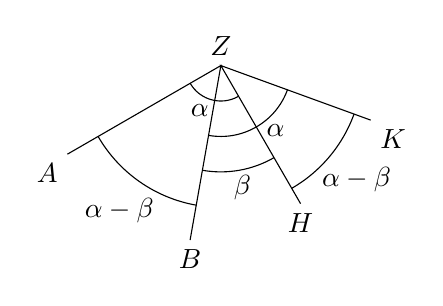
\begin{tikzpicture}[scale=.45]
\coordinate (Z) at (0,0);
\coordinate (A) at (-150:5cm);
\coordinate (B) at (-100:5cm);
\coordinate (H) at (-60:4.5cm);
\coordinate (K) at (-20:4.5cm);
\draw (A) node[below left] {$A$} -- (Z) node[above] {$Z$} -- (B) node[below] {$B$};
\draw (H) node[below] {$H$} -- (Z) -- (K) node[below right] {$K$};
\draw (-150:1cm) arc (-150:-60:1);
\draw (-100:2cm) arc (-100:-20:2);
\draw (-100:3cm) arc (-100:-60:3);
\draw (-150:4cm) arc (-150:-100:4);
\draw (-60:4cm) arc (-60:-20:4);
\node at (-115:1.4) {$\alpha$};
\node at (-50:2.4) {$\alpha$};
\node at (-80:3.5) {$\beta$};
\node at (-40:5) {$\alpha - \beta$};
\node at (-125:5) {$\alpha - \beta$};
\end{tikzpicture}
%\includegraphics[width=\textwidth]{Fig13_13b}
         \captionof{figure}{$\angle AZB=\angle HZK$.}\label{f.compass-relative4}
     \end{minipage}

\vspace{0.4cm}


$\triangle ZAB\sim\triangle ZHK$ puisque les deux sont des triangles isocèles et que nous avons montré qu'ils ont le même angle au sommet. Posons $x=\overline{HK}$. Alors 
\begin{align*}
\frac{m}{s} &= \frac{n}{x}\,,\\
x&=\frac{n}{m}s\,.\qedhere
\end{align*}

\end{proof}


%%%%%%%%%%%%%%%%%%%%%%%%%%%%%%%%%%%%%%%%%%%%%%%%%%%%%%%%%%%%%%%

\section{Construction de l'intersection de deux droites}\label{s.two-lines}

\begin{theorem}
Étant donné deux droites contenant les segments  $\overline{AB}$ et $\overline{CD}$, il est possible de construire leur intersection $S$.
\end{theorem}

\begin{proof}
Soit $C'$ et $D'$ les symétriques de $C$ et $D$ par rapport à $\overline{AB}$.
Il y a deux cas selon que $C$ et $D$ se trouvent du même côté de $\overline{AB}$ ou de côtés différents. Posons $x=\overline{CS}, c=\overline{CC'}, d=\overline{DD'}, e=\overline{CD}$ comme indiqué sur les figures~\ref{f.compass-intersection1} et \ref{f.compass-intersection2}. Nous calculons la valeur de $x$ pour chaque cas.

\textit{Cas 1:}
$C$ et $D$ sont sur des côtés différents de $\overline{AB}$.
$S$ se trouve sur $\overline{AB}$ parce que $\triangle CZS\cong \triangle C'ZS$ (deux côtés et un angle égaux) : $\overline{CZ}=\overline{C'Z}$, $\angle CZS=\angle C'ZS=90^\circ$ et $\overline{ZS}$ est un côté commun. Par conséquent, $\overline{C'S}=\overline{CS}$ et de même $\overline{D'S}=\overline{DS}$. $\triangle CSC'\sim\triangle DSD'$ sont semblables donc $\displaystyle\frac{x}{e-x} = \displaystyle\frac{c}{d}$ et la résolution de l'équation donne $x=\displaystyle\frac{c}{c+d}e$.

\begin{figure}[htbp]
\centering


\begin{tikzpicture}[scale=.9]
\coordinate (A) at (-4,0);
\coordinate (B) at (2,0);
\coordinate (C) at (-3,2);
\coordinate (D) at (1,-1);
\coordinate (Cp) at (-3,-2);
\coordinate (Dp) at (1,1);
\vertex{A};
\vertex{B};
\node[below] at (A) {$A$};
\node[below] at (B) {$B$};
\node[above] at (C) {$C$};
\node[below] at (D) {$D$};
\node[below] at (Cp) {$C'$};
\node[above] at (Dp) {$D'$};
\draw[name path=ab] ($(A)!1.3!(B)$) -- ($(B)!1.3!(A)$);
\draw[name path=cd] ($(C)!1.2!(D)$) -- ($(D)!1.1!(C)$);
\path [name intersections={of=ab and cd,by={S}}];
\node[above] at (S) {$S$};
\draw (Cp) -- node[below] {$x$} (S);
\draw (S) -- node[above,xshift=-5pt] {$e\!-\!x$} (Dp);
\draw (C) -- node[above left,yshift=6pt] {$c$} (Cp);
\draw (D) -- node[above right,yshift=6pt] {$d$} (Dp);
\path (C) -- node[right,xshift=2pt] {$x$} (S);
\path (S) -- node[left,near end,xshift=-2pt] {$e\!-\!x$} (D);
\node[below left] at (C|-A) {$Z$};
\vertex{C};
\vertex{D};
\vertex{Cp};
\vertex{Dp};
\draw ($(C)!.5!(Cp)$) rectangle +(6pt,6pt);
\draw[rotate=90] ($(D)!.5!(Dp)$) rectangle +(6pt,6pt);
\end{tikzpicture}
%\includegraphics[width=0.8\textwidth]{Fig13_14}
\caption{Construction de l'intersection de deux droites (1).}\label{f.compass-intersection1}
\end{figure}

\textit{Cas 2:}
$C$ et $D$ sont du même côté de $\overline{AB}$. $\triangle CSC'\sim DSD'$ donne $\displaystyle\frac{x}{x-e}=\frac{c}{d}\displaystyle$ et la résolution de l'équation donne $x=\displaystyle\frac{c}{c-d}e$.

\begin{figure}[htbp]
\centering
   \begin{tikzpicture}[scale=.9]
\coordinate (A) at (-4,0);
\coordinate (B) at (2,0);
\coordinate (C) at (-3,2);
\coordinate (D) at (-1,1);
\coordinate (Cp) at (-3,-2);
\coordinate (Dp) at (-1,-1);
\vertex{A};
\vertex{B};
\node[below] at (A) {$A$};
\node[below] at (B) {$B$};
\node[above] at (C) {$C$};
\node[above] at (D) {$D$};
\node[below] at (Cp) {$C'$};
\node[below] at (Dp) {$D'$};
\draw[name path=ab] ($(A)!1.3!(B)$) -- ($(B)!1.3!(A)$);
\draw[name path=cd] ($(C)!2.2!(D)$) -- ($(D)!1.1!(C)$);
\path [name intersections={of=ab and cd,by={S}}];
\node[above] at (S) {$S$};
\draw (Cp) -- (S);
\draw (C) -- node[above left,yshift=6pt] {$c$} (Cp);
\draw (D) -- node[above right,yshift=6pt] {$d$} (Dp);
\path (C) -- node[above] {$e$} (D);
\path (Cp) -- node[below] {$e$} (Dp);
\path (D) -- node[above right,xshift=-4pt] {$x-e$} (S);
\path (Dp) -- node[below right,xshift=-4pt] {$x-e$} (S);
\node[below left] at (C|-A) {$Z$};
\vertex{C};
\vertex{D};
\vertex{Cp};
\vertex{Dp};
\draw ($(C)!.5!(Cp)$) rectangle +(6pt,6pt);
\draw[rotate=90] ($(D)!.5!(Dp)$) rectangle +(6pt,6pt);
\end{tikzpicture}
%\includegraphics[width=0.9\textwidth]{Fig13_15}

\caption{Construction de l'intersection de deux droites (2).}\label{f.compass-intersection2}
\end{figure}

\medskip

Construisons les cercles $c(C',d)$ et $c(D,e)$. Soit $H$  leur intersection  (fig.~\ref{f.compass-intersection3}). La somme des segments  $\overline{CC'}$ et $\overline{C'H}$ est $c + d$. On doit montrer que $H$ est dans le prolongement de $\overline{CC'}$ pour que $\overline{CH}$ soit un segment  de longueur $c+d$. $\overline{CH} = c - d$ dans le cas où $D$ est du même côté de $\overline{AB}$ que $C$ (non représenté sur la figure).
\begin{figure}[htbp]
\centering
   \begin{tikzpicture}[scale=.8]
\coordinate (A) at (-4,0);
\coordinate (B) at (2,0);
\coordinate (C) at (-3,2);
\coordinate (D) at (1,-1);
\coordinate (Cp) at (-3,-2);
\coordinate (Dp) at (1,1);
\vertex{A};
\vertex{B};
\node[below left] at (A) {$A$};
\node[below] at (B) {$B$};
\node[above] at (C) {$C$};
\node[below] at (D) {$D$};
\node[left] at (Cp) {$C'$};
\node[above] at (Dp) {$D'$};
\draw[name path=ab] ($(A)!1.3!(B)$) -- ($(B)!1.3!(A)$);
\draw[name path=cd] ($(C)!1.2!(D)$) -- ($(D)!1.1!(C)$);
\path [name intersections={of=ab and cd,by={S}}];
\node[above,yshift=4pt] at (S) {$S$};
\draw (Cp) -- node[below right,xshift=5pt,yshift=5pt] {$e$} (Dp);
\path (C) -- node[above left] {$c$} (Cp);
\draw[thick,dashed] (D) -- node[above right] {$d$} (Dp);
\draw[name path=circled] (D) let
  \p1 = ($ (D) - (C) $),
  \n2 = {veclen(\x1,\y1)}
in
  ++(130:\n2) arc (130:230:\n2);

\draw[name path=circlecp] (Cp) let
  \p1 = ($ (D) - (Dp) $),
  \n2 = {veclen(\x1,\y1)}
in
  ++(-180:\n2) arc (-180:0:\n2);
\path [name intersections={of=circled and circlecp,by={H}}];
\node[below left] at (H) {$H$};
\draw ($(C)!1.2!(H)$) -- (C);
\draw (H) -- node[right] {$d$} (Cp);
\draw (D) -- node[right,xshift=18pt,yshift=12pt] {$e$} (H);
\vertex{Cp};
\vertex{D};
\vertex{C};
\vertex{Dp};
\vertex{H};
\path (C) -- node[above] {$x$} (S);
\path (Cp) -- node[below] {$x$} (S);
\end{tikzpicture}
%\includegraphics[width=0.8\textwidth]{Fig13_16}

\caption{Construction de l'intersection de deux droites (3).}\label{f.compass-intersection3}
\end{figure}

$H$ est l'intersection de $c(C',d)$ et $c(D,e)$, donc $\overline{DH}=e$ et  $\overline{C'H}=d$. Par construction,  $\overline{C'D'} = e$ et $\overline{D'D}=d$,  donc le quadrilatère $\overline{C'D'DH}$ est un parallélogramme. 

Par construction,  $\overline{DD'}\parallel\overline{CC'}$, donc  $\overline{C'H}\parallel \overline{DD'}$ et $\overline{C'H}\parallel\overline{CC'}$. Puisque l'une de ses extrémités est $C'$, il doit se trouver sur la droite contenant $\overline{CC'}$. D'après le théorème~\ref{thm.add-subtract-mm}, à partir des longueurs $c$, $d$ et $e$, on peut construire un segment  de longueur $c+d$ et d'après le théorème~\ref{thm.compass-ratio} on peut construire un segment  de longueur $x=\displaystyle\frac{c}{c+d}e$. L'intersection $S$ de $c(C',x)$ et $c(C,x)$ est aussi l'intersection de $\overline{AB}$ et $\overline{CD}$ (fig.~\ref{f.compass-intersection4}).
\end{proof}

\begin{figure}[thbp]
\centering
   \begin{tikzpicture}[scale=.6]
\coordinate (A) at (-4,0);
\coordinate (B) at (2,0);
\coordinate (C) at (-3,2);
\coordinate (D) at (1,-1);
\coordinate (Cp) at (-3,-2);
\coordinate (Dp) at (1,1);
\vertex{A};
\vertex{B};
\node[below left] at (A) {$A$};
\node[below] at (B) {$B$};
\node[above] at (C) {$C$};
\node[below] at (D) {$D$};
\node[left] at (Cp) {$C'$};
\node[above] at (Dp) {$D'$};
\draw[name path=ab] ($(A)!1.3!(B)$) -- ($(B)!1.3!(A)$);
\draw[name path=cd] ($(C)!1.2!(D)$) -- ($(D)!1.1!(C)$);
\path [name intersections={of=ab and cd,by={S}}];
\node[above,yshift=4pt] at (S) {$S$};
\draw (Cp) -- (Dp);
\path (C) -- node[above,yshift=4pt] {$x$} (S);
\path (Cp) -- node[below,yshift=-4pt] {$x$} (S);
\path (C) -- node[above left] {$c$} (Cp);
\draw (D) -- node[above right] {$d$} (Dp);
\draw[name path=circled] (C) let
  \p1 = ($ (S) - (C) $),
  \n2 = {veclen(\x1,\y1)}
in
  ++(-10:\n2) arc (-10:-100:\n2);

\draw[name path=circlecp] (Cp) let
  \p1 = ($ (S) - (C) $),
  \n2 = {veclen(\x1,\y1)}
in
  ++(100:\n2) arc (100:0:\n2);
\draw (Cp) -- (C);
\vertex{C};
\vertex{Cp};
\vertex{D};
\vertex{Dp};
\end{tikzpicture}
%\includegraphics[width=0.8\textwidth]{Fig13_17}

\caption{Construction de l'intersection de deux droites (4).}\label{f.compass-intersection4}
\end{figure}


%%%%%%%%%%%%%%%%%%%%%%%%%%%%%%%%%%%%%%%%%%%%%%%%%%%%%%%%%%%%%%%

\section{Construction de l'intersection d'une droite et d'un cercle}\label{s.line-circle}

\begin{theorem}
Étant donné un cercle $k=C(M,r)$ et une droite $l$, il est possible de construire les intersections de $k$ et de $l$.
\end{theorem}

\begin{proof}
Construisons le symétrique $M'$ de $M$ par rapport à $l$ et construisons le cercle $k'=c(M',r)$. Puisque $MYM'\cong\triangle MXM'$, les points $X$ et $Y$   d'intersection de $k$ et $k'$ sont les points d'intersection de $l$ et de $k$  (fig.~\ref{f.compass-circle4}).
\begin{figure}[htbp]

\centering
\begin{tikzpicture}[scale=.4]
\coordinate (A) at (-7,0);
\coordinate (B) at (8,0);
\coordinate (M) at (0,-2);
\coordinate (Mp) at (0,2);
\node[below left] at (M) {$M$};
\node[above left] at (Mp) {$M'$};
\draw[name path=c1] (M) circle[radius=3cm];
\draw[name path=c2] (Mp) circle[radius=3cm];
\draw[name path=ab] ($(A)!1.2!(B)$) --
  node[above,very near end] {$l$} ($(B)!1.2!(A)$);
\path [name intersections={of=c1 and c2,by={S1,S2}}];
\path[name path=radius1] (M) -- ++(15:4cm);
\path [name intersections={of=c1 and radius1,by={R1}}];
\draw (M) -- node[below] {$r$} (R1);
\path[name path=radius2] (Mp) -- ++(40:4cm);
\path [name intersections={of=c2 and radius2,by={R2}}];
\draw (Mp) -- node[above] {$r$} (R2);
\draw (Mp) -- (M) -- (S1) -- (Mp) -- (S2) -- (M);
\node[right,xshift=6pt,yshift=6pt] at (S1) {$X$};
\node[left,xshift=-6pt,yshift=6pt] at (S2) {$Y$};
\draw (0,0) rectangle +(10pt,10pt);
\node at (-3.5,-3) {$k$};
\node at (-3.5,3) {$k'$};
\end{tikzpicture}
%   \includegraphics[width=\textwidth]{Fig13_18}

\caption{Construction de l'intersection d'une droite et d'un cercle  (1).}\label{f.compass-circle4}
\end{figure}

Cette construction ne peut pas être faite si $M$ est sur la droite $l$. Dans ce cas, choisissons un point arbitraire $A$ sur $l$ qui est à une distance supérieure à $r$ de $M$. En utilisant le théorème~\ref{thm.add-subtract-mm}, raccourcissons et allongeons $\overline{AM}$ de $r$.  Les extrémités $X$ et $Y$  de ces segments sont les intersections de $k$ et $l$  (fig.~\ref{f.compass-circle5}).
\end{proof}

\begin{figure}[htbp]
\centering
\begin{tikzpicture}[scale=.45]
\coordinate (A) at (-7,0);
\coordinate (B) at (8,0);
\coordinate (M) at (0,0);
\vertex{M};
\vertex{A};
\node[below] at (A) {$A$};
\node[below left] at (M) {$M$};
\draw[name path=c1] (M) circle[radius=3cm];
\draw[name path=ab] ($(A)!1.2!(B)$) -- 
  node[above,very near end] {$l$} ($(B)!1.2!(A)$);
\path[name path=radius1] (M) -- ++(50:4cm);
\path [name intersections={of=c1 and radius1,by={R1}}];
\draw (M) -- node[above] {$r$} (R1);
\path [name intersections={of=c1 and ab,by={S1,S2}}];
\node[above right] at (S1) {$X$};
\node[above left] at (S2) {$Y$};
\path (M) -- node[below,xshift=4pt] {$\overline{AM}+r$} (S1);
\path (A) -- node[below] {$\overline{AM}-r$} (S2);
\node at (-2.5,2.5) {$k$};
\end{tikzpicture}
%   \includegraphics[width=\textwidth]{Fig13_19}

\caption{Construction de l'intersection d'une droite et d'un cercle  (2).}\label{f.compass-circle5}
\end{figure}




\subsection*{Quelle est la surprise ?}

Lorsqu'on apprend à construire à la règle et au compas, il semble évident que les deux outils soient nécessaires. Ce fut donc une surprise de découvrir qu'un compas est suffisant. La démonstration est assez longue, nous n'allons donc pas laisser la règle à la maison, mais le théorème montre que nous ne devrions pas supposer qu'il n'existe pas d'alternatives à des concepts mathématiques bien connus.

\subsection*{Sources}

Ce chapitre se base sur le problème $33$ de \cite{dorrie1} retravaillé par Michael Woltermann \cite{dorrie2}. Une démonstration supplémentaire se trouve dans \cite{mm}.
